\documentclass[a4paper,10pt]{report} 

\usepackage[polish]{babel}
\usepackage[utf8]{inputenc}
\usepackage{polski}
\usepackage[T1]{fontenc}

\usepackage{indentfirst}
\usepackage{amsmath, amstext} % ,amsfonts,amssymb
\usepackage{verbatim}
\usepackage{booktabs}
\usepackage{color}
\usepackage[usenames,dvipsnames,svgnames]{xcolor}
\usepackage{utopia}
\usepackage{geometry}
\geometry{verbose,lmargin=3cm,rmargin=3cm}
\frenchspacing

\usepackage{graphicx}

% podtytuł
\usepackage{titling}
\newcommand{\subtitle}[1]{
 \posttitle{
  \par\end{center}
  \begin{center}\large#1\end{center}
  \vskip0.5em}
}

%opening
\title{Nowe Trendy w Obliczeniach Neuronowych}
\subtitle{Spike and Slab Restricted Boltzmann Machine w klasyfikacji obiektów ze zbioru CIFAR-10}
\author{Konrad Brus \\ Jakub A. Gramsz}

\begin{document}
\maketitle

\begin{abstract}
Projekt ma na celu implementację Gaussian Restricted Boltzmann Machine oraz Spike and Slab RBM 
(zaprezentowanych w \cite{courville2013spike}) i wykorzystanie ich do klasyfikacji obiektów
przedstawionych na obrazach. Implementacja uczona oraz testowana będzie na zbiorze danych CIFAR-10
(przedstawiony w \cite{cifar}) przy wykorzystaniu algorytmu uczenia Contrastive Divergence.
\end{abstract}

\chapter*{}

\section{Wstęp teoretyczny}
Maszyna Boltzmanna (ang. \textit{Boltzmann Machine}, BM) jest nieskierowanym grafem probabilistycznym z
węzłami o wartościach dyskretnych lub ciągłych. Model BM można interpretować jako stochastyczną sieć
neuronową, w której stan każdego neuronu zależy od neuronów do niego połączonych. Początkowo
zaproponowano maszynę Boltzmanna jako graf pełny z neuronami o wartościach binarnych, taka sieć była
analogiczna do sieci Hopfielda jeżeli zastosowalibyśmy neurony deterministyczne zamiast stochastycznych.
Zaletą maszyny Boltzmanna nad siecią Hopfielda jest, to że maszyna Boltzmanna potrafi generować próbki
na podstawie wyuczonego rozkładu prowdopodobieństwa.

\begin{figure}
 \centering
 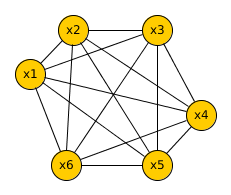
\includegraphics[width=5cm]{imgs/bm.png}
 \label{fig:bm}
\caption{Maszyna Boltzmanna, wszystkie neurony są połączone ze wszystkimi}
\end{figure} 

Szybko zauważono, że utrzymywanie wszystkich połączeń w maszynie Boltzmanna przynosi negatywne skutki.
Uczenie takiego modelu było bardzo trudne i długotrwałe, a jakość wyników nie była wystarczająco dobra
(jak na taki czas generowania modelu). Ograniczono, więc liczbę połączeń w sieci, wierzchołki podzielono
na dwie grupy warstwę widoczną i warstwę ukrytą. W nowym modelu ograniczonej maszynie Boltzmanna (ang.
\textit{Restricted Boltzmann Machine}) usunięto wszystkie połączenia pomiędzy neuronami tej samej
warstwy. Łącznie wektor wartości neuronów warstwy widocznej oznaczamy $\mathbf{x}=[x_1, x_2,\dots, x_M]$,
natomiast wektor wartości neuronów warstwy ukrytej oznaczamy przez $\mathbf{h}=[h_1, h_2,\dots, h_N]$.
Ponad to w modelu wstawia się dla każdej warstwy dodatkowy neuron zapewniający \textbf{bias}, którego
wartość jest stała i równa jeden.

\begin{figure}
 \centering
 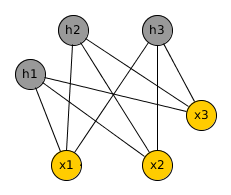
\includegraphics[width=6cm]{imgs/rbm.png}
 \label{fig:rbm}
\caption{Ograniczona maszyna Boltzmanna, połączenia występują pomiędzy wyszystkimi neuronami z różnych
warstw}
\end{figure} 

Wartosci neuronów na warstwie ukrytej traktuje się jako punkty danych, natomiast warstwa ukryta tworzy
warunkową reprezentację danych. Pozwala to na transoformacje danych do postaci warunkowej i odwrotnie.

Bardzo przydatną cechą RBM jest to, że można układać z nich stos. Możliwe jest uczenie jednego RBM na
danych z warstwy ukrytej innego. Pozwala to konstrułować sieci głębokie (ang. \textit{deep networks}).
Potrafią one uczyć się bardzo złożonych wzorców.

\section{Opis problemu}

Rozpatrywany problem można uznać za problem klasyfikacji, a więc zastosowany model można uznać ze typ
klasyfikatora. Na jego wejście podawany jest, w postaci mapy bitowej, obraz należący do jednej z klas, na
wyjściu zaś pojawia się etykieta klasy. Aby tego dokonać zestawiane są dwie ograniczone maszyny
Boltzmanna, z których pierwsza służy do ekstrakcji cech z danych wejściowych, a druga przydziela tak
otrzymane cechy do jednej z 10 klas.

Dane wejściowe warto podać pewnym procesom przetwarzania wstępnego. Pierwszym z nich jest podział na segmenty, w którym obraz dzielony jest na małe regiony w pewien ustalony sposób. Przyjeliśmy metodę podziału na 25 takich regionów, przedstawioną na rys 3.

\begin{figure}
 \centering
 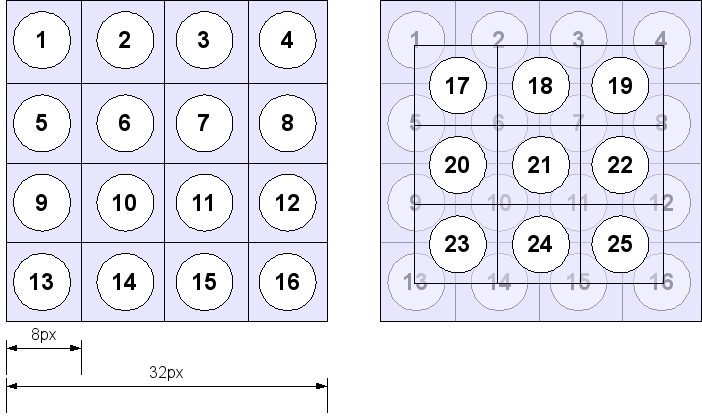
\includegraphics[width=6cm]{imgs/segmentacja.png}
 \label{fig:segmentacja}
 \caption{Podział obrazka 32x32 piksele na 25 regionów o wymiarach 8x8 pikseli \cite{cifar}}
\end{figure}

Segmenty takie poddawane są następnie tzw. centeringowi, który zapewnia, że średnia każdego z nich jest bliska lub równa 0.

Ponieważ obrazy, w szczególności te o niewielkich rozmiarach, wykazują dużą korelację między sąsiednimi pikselami, warto takie powiązania usunąć za pomocą transfomacji wybielania (whitening) danych, by ułatwić modelowi wyuczenie się cech wyższego poziomu. W efekcie zachowywane są krawędzie zawarte na obrazie, a regiony podobne kolorystycznie są zerowane. Przedstawiono to na rys 4.

\begin{figure}
 \centering
 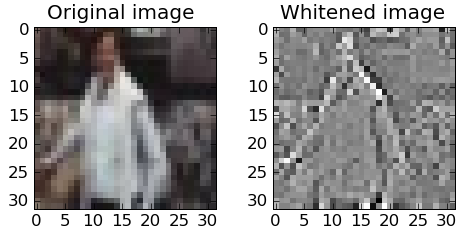
\includegraphics[width=6cm]{imgs/whitening.png}
 \label{fig:whitening}
 \caption{Efekt transformacji wybielającej \cite{melchior2012}}
\end{figure}

\section{Opis modelu}

Podstawową wersją ograniczonej maszyny Boltzmanna jest odmiana BB-RBM (Binary-Binary RBM). Składa się ona z warstwy binarnych jednostek widocznych oraz binarnych jednostek ukrytych, co wymusza binarną reprezentację danych wejściowych $\mathbf{x}$ i skutkuje binarną reprezentacją ukrytą $\mathbf{h}$. W takiej formie, każda jednostka widoczna $v_i$ oraz ukryta $h_j$ posiadają, odpowiednio, wejścia bias $b_i^v$ oraz
$b_j^h$. Jednostka ukryta z widoczną połączone są wagami $w_ij$.

Dla modelu RBM definuje się funkcję energii \textbf{E}, określoną:

\begin{align}
	\mathbf{E_{BB-RBM}(v,h) = - \sum_{i=1}^{V} \sum_{j=1}^{H} v_i h_j w_ij - \sum_{i=1}^{V} v_i b_i^v - \sum_{j=1}^{H} h_j b_j^h}
\end{align}

Nie jest to najbardziej intuicyjne podejście w przypadku modelowania obrazów (i, w ogólności, danych pochodzących z dziedziny rzeczywistej), co umotywowało utworzenie wersji RBM, w której warstwa ukryta jest w dalszym ciągu binarna, lecz warstwa widoczna jest ciągła, o rozkładzie normalnym, średniej $b_i$ i wariancji $\sigma^2_i$. Odmiana taka to GB-RBM (Gaussian-Binary RBM).

Z taką odmianą skojarzona jest następująca funkcja energii:

\begin{align}
	\mathbf{E(v,h) = \sum_{i=1}^{V} \frac{(v_i - b_i^v)^2}{2\sigma_i^2} - \sum_{j=1}^{H} b_j^h h_j - \sum_{i=1}^{V} \sum_{j=1}^{H} \frac{v_i}{\sigma_i} h_j w_ij}
\end{align}

\section{Opis algorytmu uczenia}

Prawdopodobieństwo wystąpienia pewnej konfiguracji $(v, h)$ opisywane jest 

\begin{align}
	\mathbf{p(v,h) = \frac{e^{-E(v,h)}}{\sum_x \sum_k e^{-E(x,k)}}}
\end{align}

\textbf{u} oraz \textbf{k} oznaczają tutaj przestrzeń wszystkich możliwych konfiguracji jednostek ukrytych i widocznych, zatem suma występująca w mianowniku jest trudna do obliczenia.

Ze wzoru wynika również, że konfiguracje o wysokiej energii mają niższe prawdopodobieństwo wystąpienia niż konfiguracje o niskiej energii.

W ogólności, procedura uczenia ograniczonej maszyny Boltzmanna polega na ustaleniu stanów jednostek ukrytych w pewnej ich konfiguracji i odnalezieniu takich wartości parametrów wag i parametrów \textit{bias}, by prawdopodobieństwo wystąpienia danej konfiguracji \textbf{v} było duże. Wykorzystuje się do tego celu metodę gradientu prostego.

\begin{align}
 \mathbf{\sum^{C} log p(v^c) = \sum^{C} log \frac{\sum_g e^{-E(v^c, g)}}{\sum_u \sum_g e^{-E(u,g)}}}
\end{align}

Różniczkując, otrzymujemy:

\begin{align}
 \mathbf{\frac{\partial}{\partial w_ij} \sum^{C} log p(v^c) = \frac{\partial}{\partial w_ij} \left(  \sum^C log \sum_g e^{-E(v^c, g)} - log \sum_u \sum_g e^{-E(u,g)} \right)}
\end{align}

Ponieważ wartość tego wyrażenia można obliczyć jedynie przez nieskończone powtarzanie procesu samplowania na przemian warstw widocznej i ukrytej, do przybliżenia jej stosuje się algorytm oparty na optymalizacji funkcji tzw. \textit{contrastive divergence}, która taki ciąg przeprowadza tylko kilka razy.

\begin{figure}
 \centering
 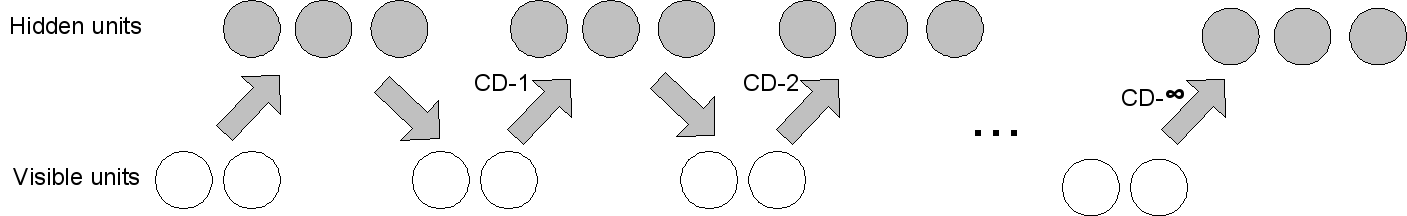
\includegraphics[width=10cm]{imgs/cd-n.png}
 \label{fig:contrastivedivergence}
 \caption{Przebieg procedury CD \cite{cifar}}
\end{figure}

\section{Opis eksperymentu i zbioru danych}
Do badań zostanie użyty zbiór CIFAR-10. Zawiera on 60000 kolorowych obrazów o wymiarach 32x32 pikseli, należących do jednej z 10 klas: 
\begin{itemize}
	\item airplane, automobile, bird \\
	\begin{center} 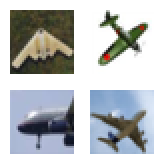
\includegraphics{imgs/class_0.png} 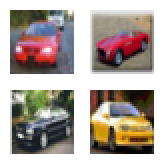
\includegraphics{imgs/class_1.png} 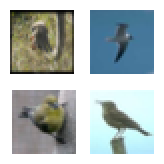
\includegraphics{imgs/class_2.png} \end{center}

	\newpage

	\item cat, deer, dog \\
	\begin{center} 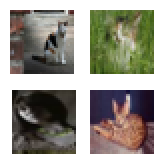
\includegraphics{imgs/class_3.png} 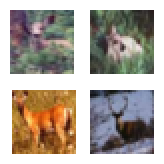
\includegraphics{imgs/class_4.png} 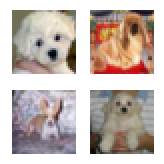
\includegraphics{imgs/class_5.png} \end{center}

	\item frog, horse, ship \\
	\begin{center} 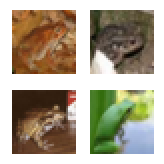
\includegraphics{imgs/class_6.png} 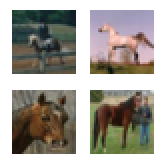
\includegraphics{imgs/class_7.png} 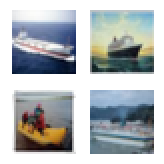
\includegraphics{imgs/class_8.png} \end{center}

	\item truck \\
	\begin{center} 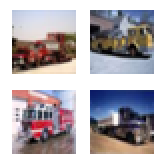
\includegraphics{imgs/class_9.png} \end{center}
\end{itemize}

Na jedną klasę przypada 6000 obrazów.

Zbiór jest wstęnie podzielony na dwie części - treningową (zawierającą 50000 obrazów, 5000 na klasę) oraz testową (10000 obrazów, 1000 na klasę).



Eksperyment zaplanowany jest następująco:

\begin{itemize}
	\item utworzenie 25 modeli GB-RBM o \textit{n}, trenowanych niezależnie na każdym z segmentów powstałych po wstępnym przetworzeniu danych (n jest tutaj parametrem, który może podlegać pewnemu dostrojeniu),
	\item utworzenie nadrzędnego modelu RBM o $\textit{n} \times 25$ jednostkach ukrytych, inicjowanych wagami kolejnych modeli niższego poziomu,
	\item sprawdzenie, czy zmiana rozmiaru segmentów ma wpływ na skuteczność rozpoznawania obiektów.
\end{itemize}

\bibliographystyle{abbrv}
\nocite{*} % na razie póki mało co jest cytowane (powoduje że wszystko z listy artykułów jest tu widoczne
\bibliography{lit}

\end{document}
